\chapter{実験 : MNISTを用いた予備実験}

\section{概要}
本章では,本研究で提案するQuery-By-Dropout-Predictionsの有効性を検証するためにMNISTに対して行った実験について説明する.
Dropoutによってサンプリングされた各部分ネットワークの出力が未知データに対して分散を持つのかを検証し,
それらをCommitteeとして扱いその予測の不一致度を利用することが能動学習のクエリ選考基準として有効であるかを確認する.


\section{実験設定}

\subsection{データセットについて}
MNISTは28×28ピクセルの手書き数字のデータセットである.
7万枚の画像からなり,そのうちの6万枚は訓練画像,残りの1万枚はテスト画像として利用される.
それぞれの画像は0〜9までの数字ラベルが割り当てられているが,能動学習の状況を再現するため,
クエリとして問い合わせられるまではラベルへのアクセスが与えられない状況を設定する.


\subsection{実験の詳細}

識別器にはCNNを利用する.その構造を表\ref{table:mnist_cnn}に示す.
比較的小さなCNNであるため,クエリ問い合わせによってラベルが追加されるごとにモデルのパラメータを初期値に戻して再学習を行うことにする.
ただし毎回ランダムに初期化するのではなく,同じ初期値を利用することにする.
これは,本来各iterationでクエリとして選択されるのはその時点でのモデルにとって有効なサンプルであり,
パラメータを初期化するとそれらの重要度が変化してしまうという問題を少しでも緩和するためである.

使用するCNNは多層ニューラルネットワークの中では小さいモデルではあるものの,ラベルを1つずつ追加して再学習を行うのは計算コストが大きいため,バッチ型能動学習を採用する.
ここでも,同一クエリ内での情報の重複を避けるためクラスタリングを行う.
MNISTは画像1枚あたり784次元の比較的小さいデータであるため,元の画像情報をそのまま特徴量としてk-meansによるクラスタリングを行う.
Committeeサイズは10,k-meansのクラスター数$K$は100,再学習のepoch数は100に設定した.
一度に選択するクエリ$\mathcal{Q}$のサイズは5, 10, 50の3通りを実験した.
また,クラスターの代表サンプルから無作為にサンプリングされた20個のサンプルをラベルを付与して学習初期のラベルつきデータとして実験を開始した.
訓練時にはcrop領域をランダムにずらすRandom Crop Augmentationを利用した.
各クエリ問い合わせ毎に10000枚のテストデータに対する識別精度を計測し,ラベルを付与されたデータが1000枚に到達するまで実験を続けた.
実験ごとのばらつきを考慮し,同一の実験を3回行いその平均と標準偏差を計算した.

\begin{table}[h]
    
    \caption{\label{table:mnist_cnn}MNISTの実験に使用したCNNの構造を示す.(Kerasのexampleプログラムを参考にした.)}
    \center
    \begin{tabular}{|c|c|c|c|} \hline
        layer & size & activation & dropout ratio\\ \hline
        Convolution & $32 \times 4 \times 4$ & relu & - \\
        Convolution & $32 \times 4 \times 4$ & relu & - \\
        Max Pooling & $2 \times 2$ & - & 0.25  \\ 
        Fully Connected & 128 & relu & 0.5 \\
        Fully Connected & 128 & relu & - \\
        \hline
    \end{tabular}
\end{table}

\subsection{比較手法について}
提案するQuery-By-Dropout-Predictionsの性能を比較するため,いくつかの手法について実験を行った.
クエリの選考基準以外は全ての設定を揃えて実験を行った.
Random Sampling以外はクラスタリングによるクエリの情報重複の回避を行った.

\subsubsection{Random Sampling}
この実験のベースラインとなる選択基準.各クエリ問い合わせ毎にランダムに$\mathcal{U}$からサンプルを選択してラベル付きデータセットに追加する.

\subsubsection{Uncertainty Sampling}
推論時にDropoutを使用せずに単一の予測分布のエントロピーを利用する.
\begin{eqnarray}
    score(x) =  - \sum_i {P_{\theta}(y_i|x)} \log P_{\theta}(y|x)
\end{eqnarray}

\subsubsection{Query-By-Dropout-Predictions $+$ Uncertain Sampling}
推論時にDropoutを利用し,複数のpredictionを出力しそれらの平均の不確かさと不一致度を基準として利用する.
不確かさには予測分布のエントロピー(Entropy Sampling)を利用する.
不一致度にはCommitteeの予測分布のAverage Kullback–Leibler Divergenceを利用する.
\begin{eqnarray}
    score(x) =  -  \frac{1}{C} \sum_{c=i}^C KL \, (P_{\theta^{(c)}} || P_C) \, - \sum_i {P_C(y_i|x)} \log P_C(y|x)
\end{eqnarray}

\subsubsection{Query-By-Dropout-Predictions $+$ Uncertain Sampling $+$ 推論時Data Augmentation}
上記のクエリ基準に加え,推論時にもData Augmentationを利用することで特徴抽出層の学習に有効だと考えられるサンプルも選択できるようにする.
% \subsubsection{Dropoutにより周辺化した予測分布を利用したUncertainty Sampling}
% 推論時にDropoutを使用せずに単一の予測分布のエントロピーを利用する.\todo{このへんあやしいベイズCNNの話しないと}
% \begin{eqnarray}
%     score(x) =  - \sum_i {P_C(y_i|x)} \log P_C(y|x)
% \end{eqnarray}


\section{予備実験}
Query-By-Dropout-Predictionsによって適切なクエリを選択できるするためには,Dropoutによって元のネットワークからサンプリングされた部分ネットワークが
そのバージョン空間を近似的に表現していなければならない.
すなわち,各Commiteeが訓練データに対してはConsistentであり,未知データに対してそれぞれの予測同士に分散を持つことが必要となる.
この予備実験ではこれを示す.
ランダムに$1000$サンプルを選択しラベルを付与して学習を行った後,
訓練データ,未知データに対するCommitteeの各メンバの識別精度,それらの予測の不一致度をそれぞれ計算した.
結果を表\ref{table:mnist_pre_experiment}に示す.

\begin{table}[h!]
    \caption{\label{table:mnist_pre_experiment}Dropoutからサンプリングされた部分ネットワークの予測を計測した実験の結果}
    \center
    \subfloat[識別精度]{
        \begin{tabular}{c|c|c} \hline
            & 訓練データ & 未知データ \\ \hline \hline
            Full Network & 100.0 $\%$ & 97.8 $\%$ \\ \hline
            Committee 1 & 99.4 $\%$ & 96.4 $\%$ \\
            Committee 2 & 99.7 $\%$ & 96.4 $\%$ \\
            Committee 3 & 99.5 $\%$ & 96.3 $\%$ \\
            Committee 4 & 99.3 $\%$ & 96.4 $\%$ \\
            Committee 5 & 99.5 $\%$ & 96.4 $\%$ \\
            Committee 6 & 99.5 $\%$ & 96.4 $\%$ \\
            Committee 7 & 99.8 $\%$ & 96.4 $\%$ \\
            Committee 8 & 99.2 $\%$ & 96.3 $\%$ \\
            Committee 9 & 99.1 $\%$ & 96.5 $\%$ \\
            Committee 10 & 98.7 $\%$ & 96.4 $\%$ \\
           \hline
       \end{tabular}
    }
    \vspace{0.5cm}

    \subfloat[不一致度]{
        \begin{tabular}{c|c|c} \hline
            & 訓練データ & 未知データ \\ \hline
           Average KL & 0.027 $\pm$ 0.061 & 0.052 $\pm$ 0.12 \\
           Vote Entropy & 0.019 $\pm$ 0.087 & 0.060 $\pm$ 0.19 \\
           \hline
       \end{tabular}
    }
\end{table}

表から,Dropoutからサンプリングされた部分ネットワークは訓練データに対してはConsistentであり
未知データに対する予測はそれぞれ分散を持つことがわかる.
よって,これらの部分ネットワークをQuery-By-CommitteeのCommitteeとして利用するのは妥当であると考えられる.

\clearpage

\section{実験結果}
本項では上述した実験の結果を示す.
クエリ選考基準として提案手法,比較手法それぞれを使用した際の,ラベル付きサンプル数の増加に対するテスト精度の変化のグラフを図\ref{fig:mnist_acc_graph}に示す.
また,テストデータの識別精度が$90\%$,$95\%$,$98\%$を超えるのに要したラベルの数を表\ref{table:mnist_samplenum_accuracy}に示す.
提案した手法がUncertain Samplingのみを使用した場合と比較して性能が良いことがわかる.
これは上記に述べた通り多層ニューラルネットワークが正しくモデルの不確かさを表現できていないからだと推測される.
さらに,推論時にもData Augmentationを利用することで,さらに少ないラベルで高精度を達成していることがわかる.
それぞれのクエリ選考基準を利用して構築された1000枚のラベル付きデータセットを学習した識別精度と,ラベルを全て使った場合の識別精度の比較した図を表\ref{table:mnist_last_accuracy}に示す.
表より,提案手法を用いた場合,全てのラベルを利用して達成される識別精度に匹敵する性能を,それらの約$2\%$のラベル数で達成できていることがわかる.

また,ラベル付きデータセットが100枚の際に,各手法によってクエリとして選択されたサンプルを図\ref{figure:mnist_query_examples}に示す.
Random Sampling以外の手法は,Random Samplingと比較すると認識が困難であると考えられるサンプルを選択する傾向にある.
Uncertain Samplingではクラスタリングを行っているものの,数字の4を含むクラスターは10以上あるため,
偶然数字の4が極端に曖昧であったときに図のようなクエリになってしまうと考えられる.
さらに,画像の中間特徴量を2次元にt-SNEによって射影し,Uncertain Sampling, QBDPによってそれぞれどのサンプルが選択されているかを表した(図\ref{fig:mnist_scatter}).
提案手法はUncertain Samplingと比較すると不確かなだけでなく,識別面を大きく変え得るサンプルを好む傾向にあることがわかる.

% \begin{figure}[hbp]
%     \begin{center}
%         \subfloat[$k=5$]{
%           \scalebox{0.8}{
%             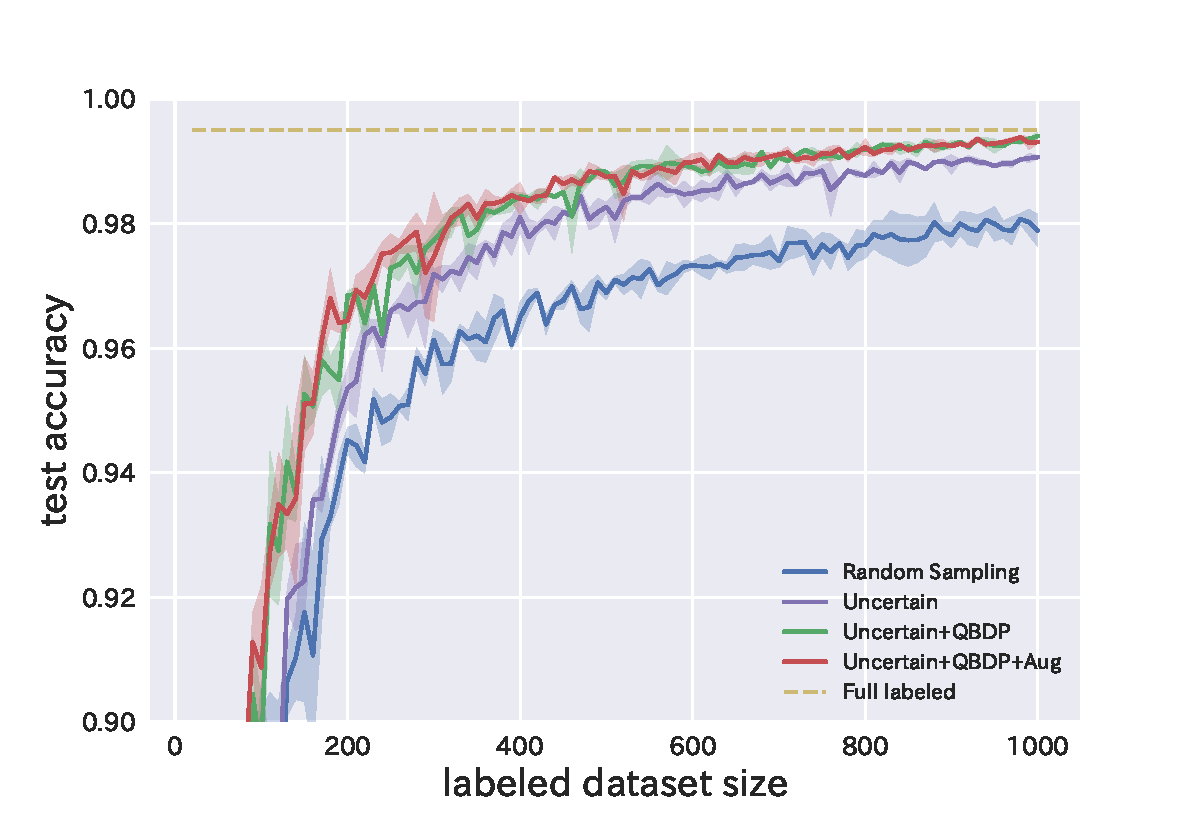
\includegraphics[width=12cm]{figures/mnist_acc_graph.pdf}
%             }
%         }

%         \vspace{0.1cm}
%         \subfloat[$k=10$]{
%         \scalebox{0.8}{
%             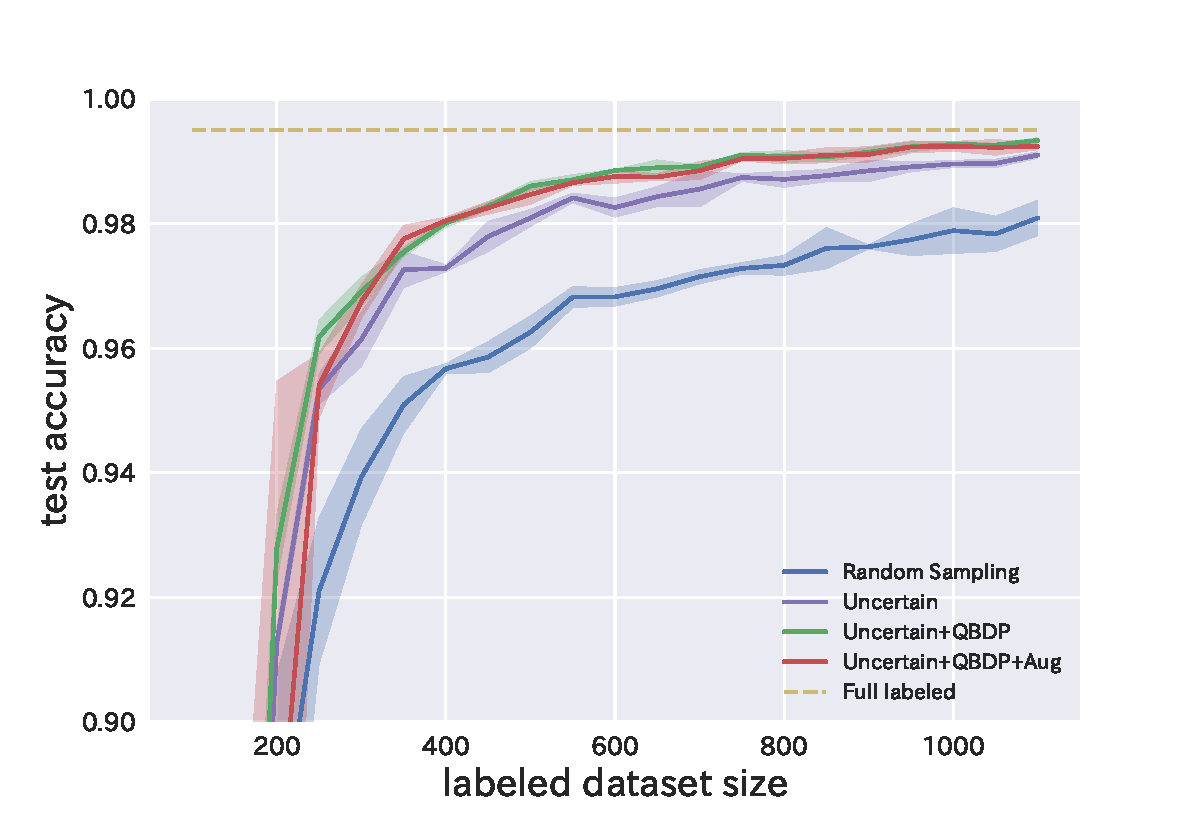
\includegraphics[width=12cm]{figures/mnist_acc_graph_50.pdf}
%           }
%         }
%         \vspace{0.1cm}
%         \subfloat[$k=50$]{
%         \scalebox{0.8}{
%             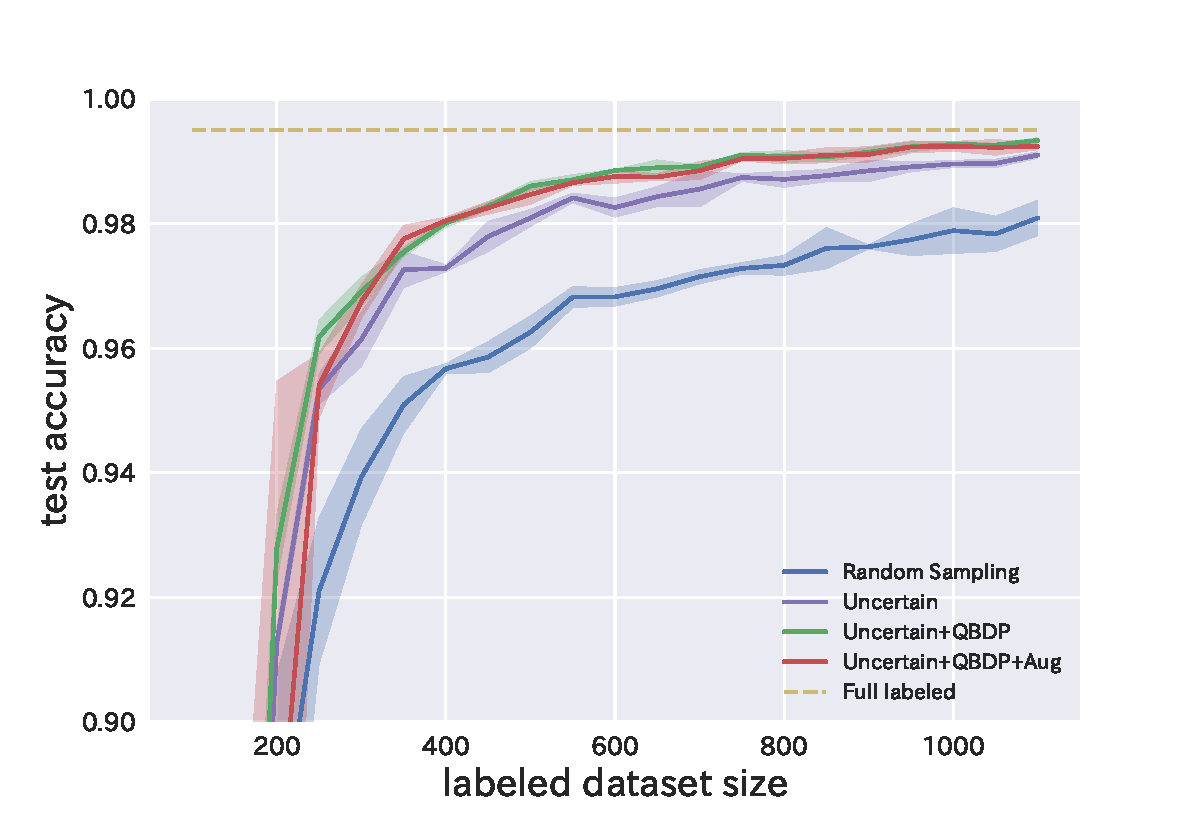
\includegraphics[width=12cm]{figures/mnist_acc_graph_50.pdf}
%           }
%         }

%         \caption{\label{fig:mnist_acc_graph}各手法を利用した場合のラベル付きサンプル数の増加に対するテスト精度の変化を示した図}
%     \end{center}
% \end{figure}

\begin{figure}[h]
     \begin{center}
      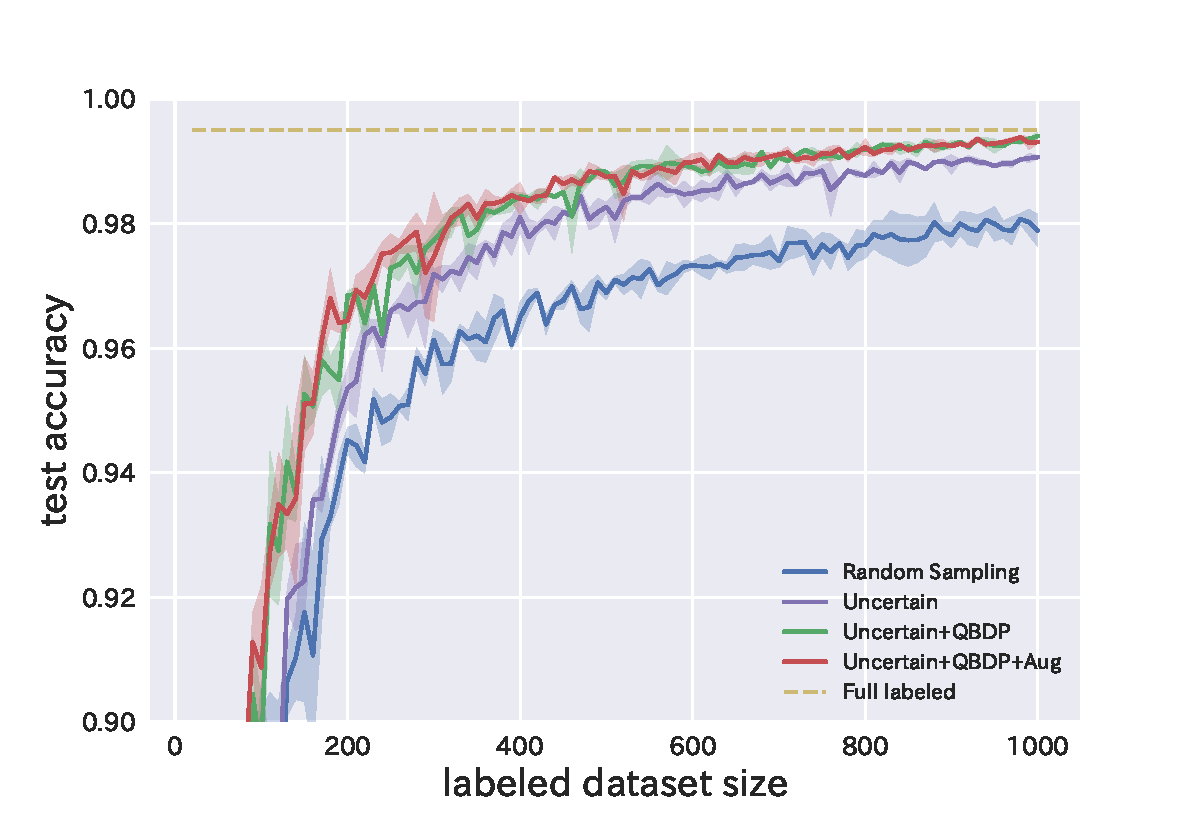
\includegraphics[width=12cm]{figures/mnist_acc_graph.pdf}
     \end{center}
    \caption{\label{fig:mnist_acc_graph}各手法を利用した場合のラベル付きサンプル数の増加に対するテスト精度の変化を示した図($k=10$)}
\end{figure}


\begin{figure}[hbp]
    \begin{center}
        \subfloat[$k=5$]{
            \begin{tabular}{c|c|c|c} 
                & $90\%$ & $95\%$ & $98\%$ \\ \hline
               Random & 110 $\pm$ 15 & 230 $\pm$ 22 & 900 $\pm$ 100 \\
               Uncertain Sampling & 100 $\pm$ 5 & 170 $\pm$ 20  & 380 $\pm$ 25 \\
               Uncertain + QBDP & 80 $\pm$ 5 & 140 $\pm$ 20 & \textbf{290} $\pm$ 10 \\ 
               Uncertain + QBDP + Aug & 70 $\pm$ 15 & 140 $\pm$ 10 & 295 $\pm$ 30 \\
           \end{tabular}
        }
        \vspace{0.1cm}
        \subfloat[$k=10$]{
            \begin{tabular}{c|c|c|c} 
                & $90\%$ & $95\%$ & $98\%$ \\ \hline
               Random & 110 $\pm$ 20 & 240 $\pm$ 10 & 900 $\pm$ 70 \\
               Uncertain Sampling & 130 $\pm$ 5 & 180 $\pm$ 20  & 420 $\pm$ 30 \\
               Uncertain + QBDP & 100 $\pm$ 10 & 150 $\pm$ 20 & 320 $\pm$ 10 \\ 
               Uncertain + QBDP + Aug & 90 $\pm$ 0 & 150 $\pm$ 5 & \textbf{300} $\pm$ 30 \\
       
           \end{tabular}
        }
        \vspace{0.1cm}
        \subfloat[$k=50$]{
            \begin{tabular}{c|c|c|c} 
                & $90\%$ & $95\%$ & $98\%$ \\ \hline
               Random & 150 $\pm$ 25 & 300 $\pm$ 25 & 900 $\pm$ 50 \\
               Uncertain Sampling & 120 $\pm$ 0 & 170 $\pm$ 0  & 435 $\pm$ 25 \\
               Uncertain + QBDP & 120 $\pm$ 0 & 170 $\pm$ 0 & 350 $\pm$ 25 \\ 
               Uncertain + QBDP + Aug & 140 $\pm$ 25 & 190 $\pm$ 25 & \textbf{320} $\pm$ 40 \\
           \end{tabular}
        }
        \caption{\label{table:mnist_samplenum_accuracy}それぞれのクエリ選考基準を利用した場合にテスト精度を達成するために要したラベルの数}
    \end{center}
\end{figure}

% \begin{table}[h]
%     \caption{\label{table:mnist_samplenum_accuracy}それぞれのクエリ選考基準を利用した場合にテスト精度を達成するために要したラベルの数}
%     \center
%     \begin{tabular}{c|c|c|c} 
%          & $90\%$ & $95\%$ & $98\%$ \\ \hline
%         Random & 110 $\pm$ 20 & 240 $\pm$ 10 & 900 $\pm$ 70 \\
%         Uncertain Sampling & 180 $\pm$ 5 & 270 $\pm$ 20  & 600 $\pm$ 50 \\
%         Uncertain + QBC + Clustering & 100 $\pm$ 10 & 150 $\pm$ 20 & 320 $\pm$ 10 \\ 
%         Uncertain + QBC + Clustering + DA & 90 $\pm$ 0 & 150 $\pm$ 5 & 300 $\pm$ 30 \\

%     \end{tabular}
% \end{table}


\begin{figure}[hbp]
    \begin{center}
        \subfloat[$k=5$]{
            \begin{tabular}{c|c} 
                &  識別精度 \\ \hline
               Random & 98.1 ± 0.3  $\%$ \\
               Uncertain Sampling & 99.2 ± 0.1 $\%$  \\
               Uncertain + QBDP & 99.3 ± 0.1  $\%$ \\ 
               Uncertain + QBDP + Aug & \textbf{99.4} ± 0.0  $\%$ \\ \hline
               Full label (60000 label) & 99.5 $\%$
           \end{tabular}
        }
        \vspace{0.1cm}
        \subfloat[$k=10$]{
            \begin{tabular}{c|c} 
                &  識別精度 \\ \hline
               Random & 97.9 ± 0.3  $\%$ \\
               Uncertain Sampling & 99.1 ± 0.0 $\%$  \\
               Uncertain + QBDP & \textbf{99.3} ± 0.1  $\%$ \\ 
               Uncertain + QBDP + Aug & \textbf{99.3} ± 0.0  $\%$ \\ \hline
               Full label (60000 label) & 99.5 $\%$
           \end{tabular}
        }
        \vspace{0.1cm}
        \subfloat[$k=50$]{
            \begin{tabular}{c|c} 
                &  識別精度 \\ \hline
               Random & 98.0 ± 0.1  $\%$ \\
               Uncertain Sampling & 99.1 ± 0.0 $\%$  \\
               Uncertain + QBDP & \textbf{99.3} ± 0.0  $\%$ \\ 
               Uncertain + QBDP + Aug & \textbf{99.2} ± 0.1  $\%$ \\ \hline
               Full label (60000 label) & 99.5 $\%$
           \end{tabular}
        }

        \caption{\label{table:mnist_last_accuracy}それぞれのクエリ選考基準を利用して構築された1000枚のラベル付きデータセットを学習した識別精度と,ラベルを全て使った場合の識別精度の比較}
    \end{center}
\end{figure}


% \begin{table}[h]
%     \caption{\label{table:mnist_last_accuracy}それぞれのクエリ選考基準を利用して構築された1000枚のラベル付きデータセットを学習した識別精度と,ラベルを全て使った場合の識別精度の比較}
%     \center
%     \begin{tabular}{c|c} 
%          &  識別精度 \\ \hline
%         Random & 97.9 ± 0.3  $\%$ \\
%         Uncertain Sampling & 99.1 ± 0.0 $\%$  \\
%         Uncertain + QBC + Clustering & 99.3 ± 0.1  $\%$ \\ 
%         Uncertain + QBC + Clustering + DA & 99.3 ± 0.0  $\%$ \\ \hline
%         Full label (60000 label) & 99.5 $\%$
%     \end{tabular}
% \end{table}


\begin{figure}[hbp]
    \begin{center}
        \subfloat[Random Sampling]{
          \scalebox{0.8}{
            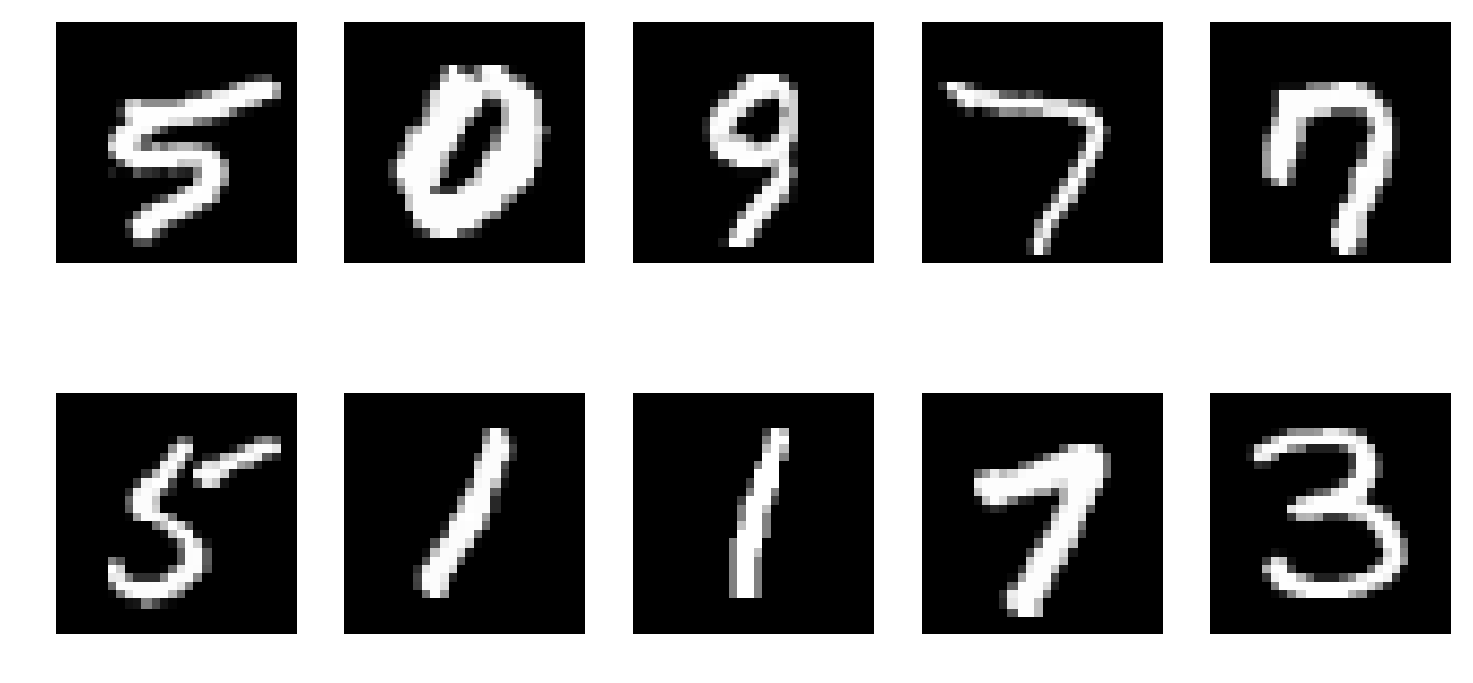
\includegraphics[width=8cm]{figures/mnist_query_example_Random.pdf}
            }
        }
        \subfloat[Uncertain Sampling]{
          \scalebox{0.8}{
            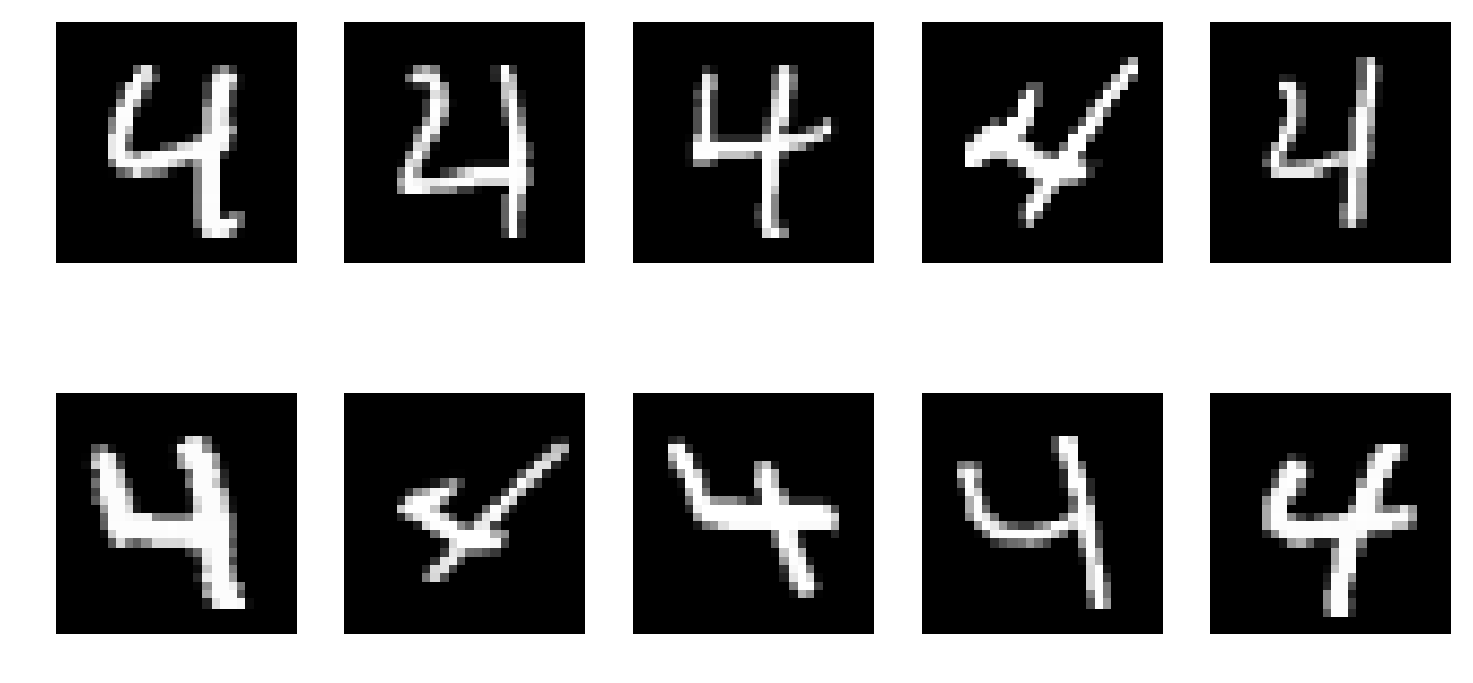
\includegraphics[width=8cm]{figures/mnist_query_example_Uncertain.pdf}
          }
        }
        \vspace{0.5cm}
        \subfloat[Uncertain + QBDP]{
        \scalebox{0.8}{
            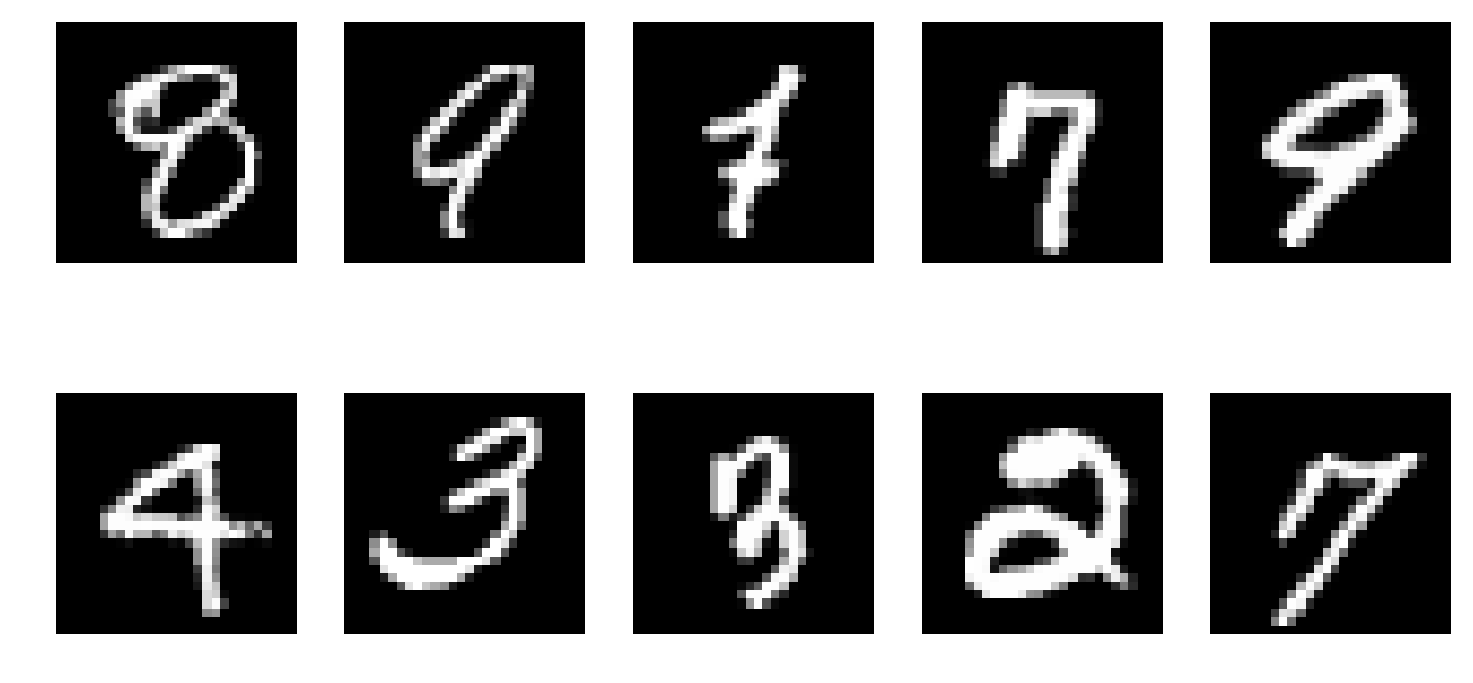
\includegraphics[width=8cm]{figures/mnist_query_example_Uncertain+QBDP.pdf}
          }
        }
        \subfloat[Uncertain + QBDP + Aug]{
        \scalebox{0.8}{
        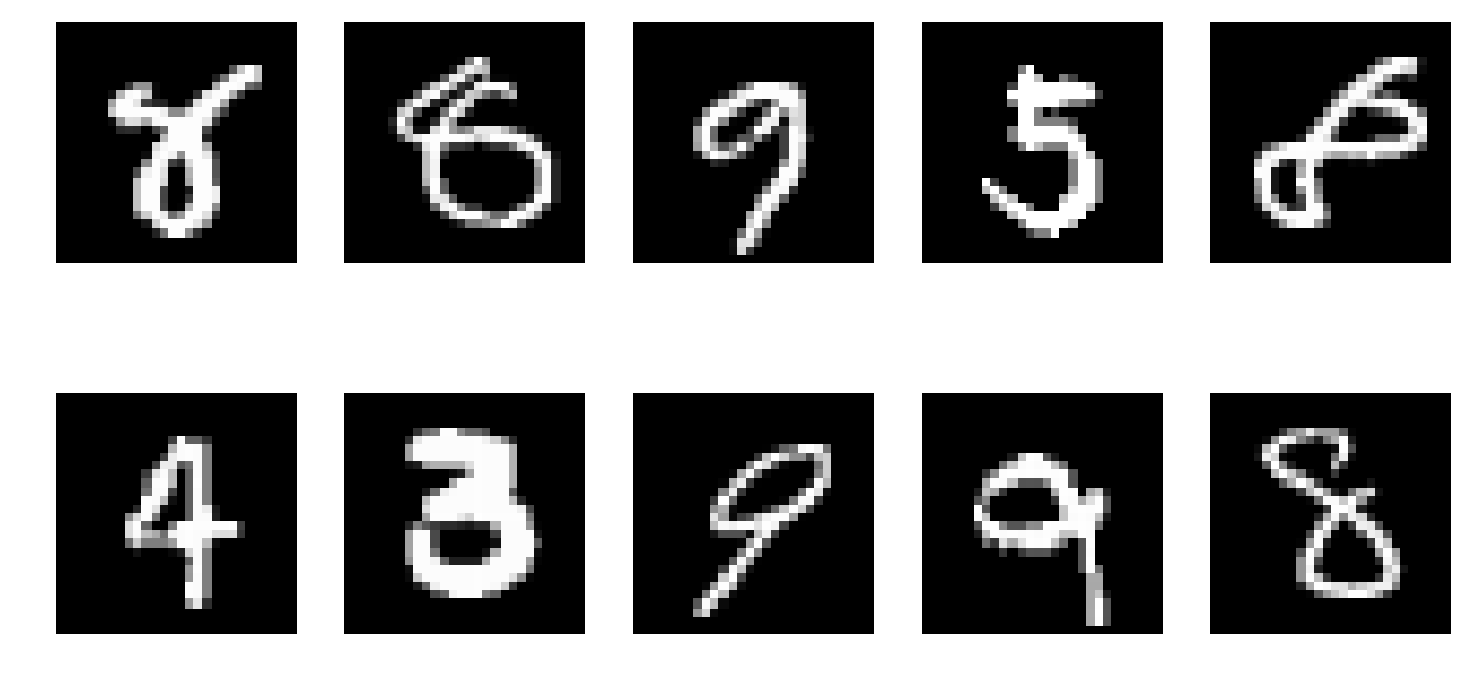
\includegraphics[width=8cm]{figures/mnist_query_example_Uncertain+QBDP+AugOnInference.pdf}
            }
        }
    \caption{\label{figure:mnist_query_examples}各手法によってクエリとして選択されたサンプルの例.}
    \end{center}
\end{figure}

\begin{figure}[h]
    \begin{center}
     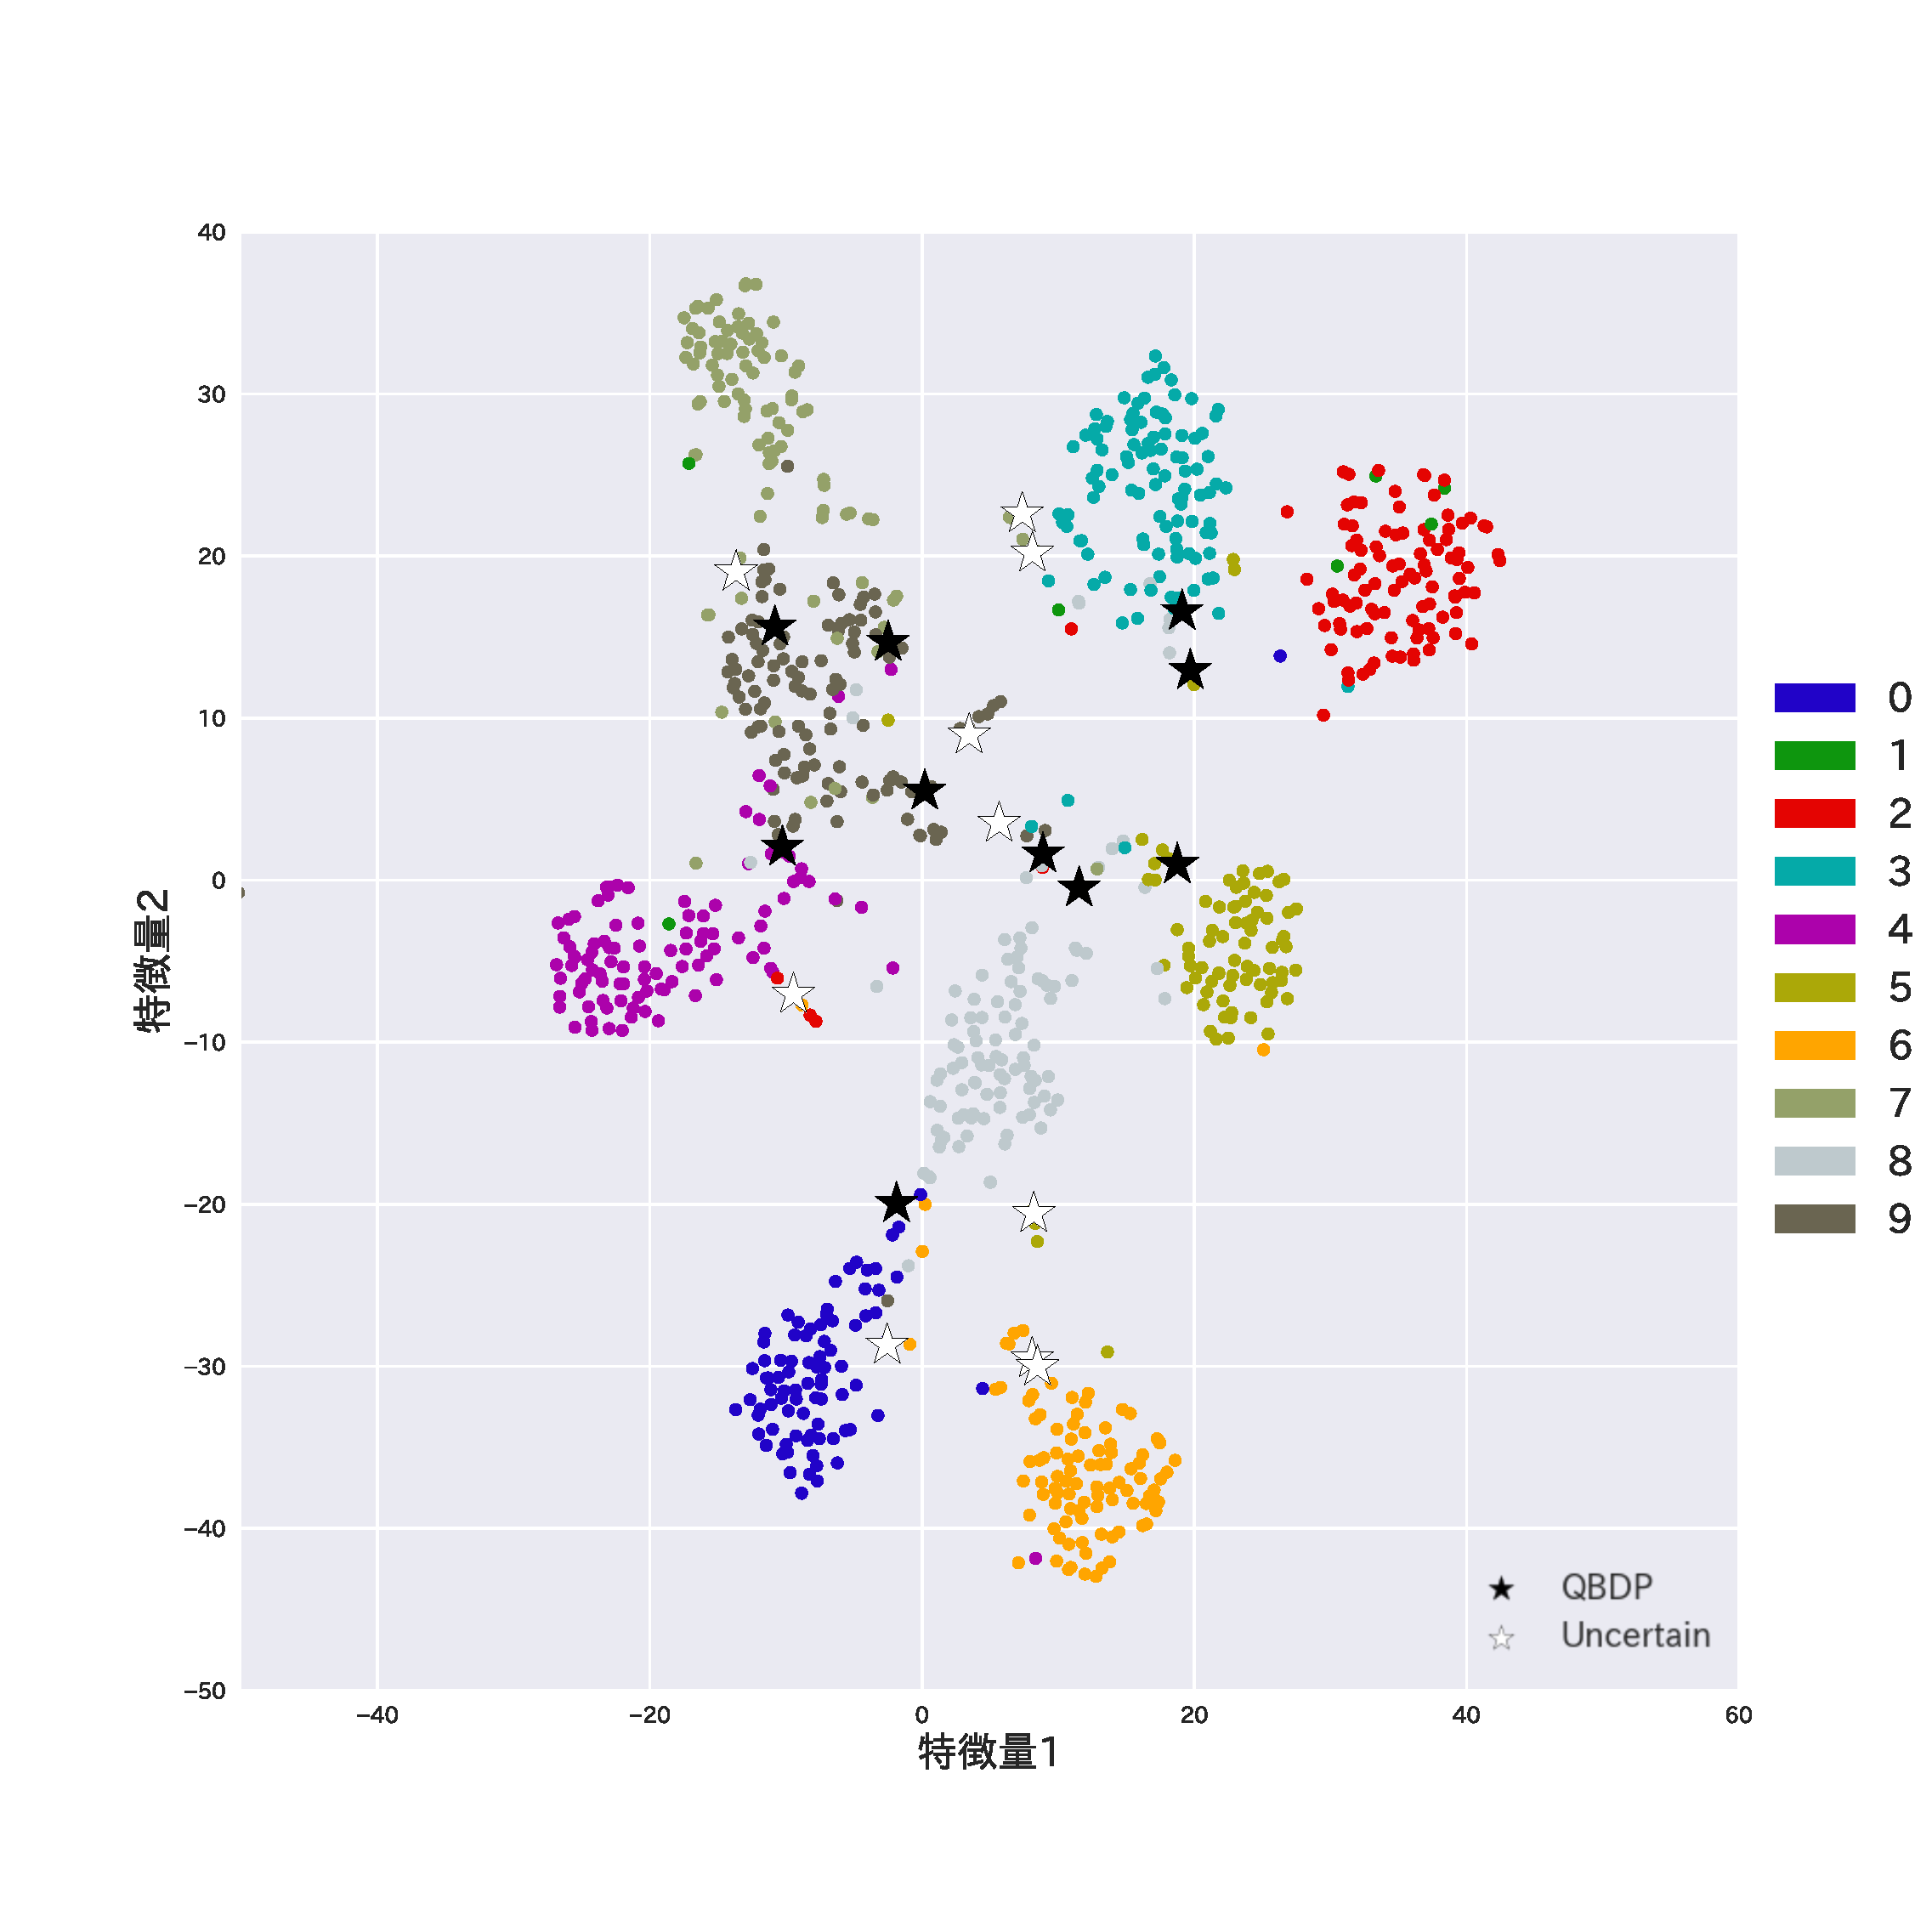
\includegraphics[width=12cm]{figures/mnist_scatter.pdf}
    \end{center}
   \caption{\label{fig:mnist_scatter}サンプルの中間特徴量を2次元にt-SNEによって射影し,各手法によってどのサンプルが選択されているかを表した図.}
\end{figure}

\clearpage

\section{まとめ}
本研究で提案するQuery-By-Dropout-PredictionsをMnistで検証し,その有効性を確認した.
全てのラベルを利用した際の
部分ネットワークが適切にバージョン空間を近似し,それを縮小させるサンプルを選択できていると考えられる.
また,非常に簡単なData Augmentationを追加することでわずかではあるが性能が向上したことから,
病理画像での複雑なData Augmentationを利用する場合は,さらに性能に変化が現れることが期待される.
